\documentclass{standalone}
\usepackage{tikz}
\usetikzlibrary{patterns, positioning}


\begin{document}
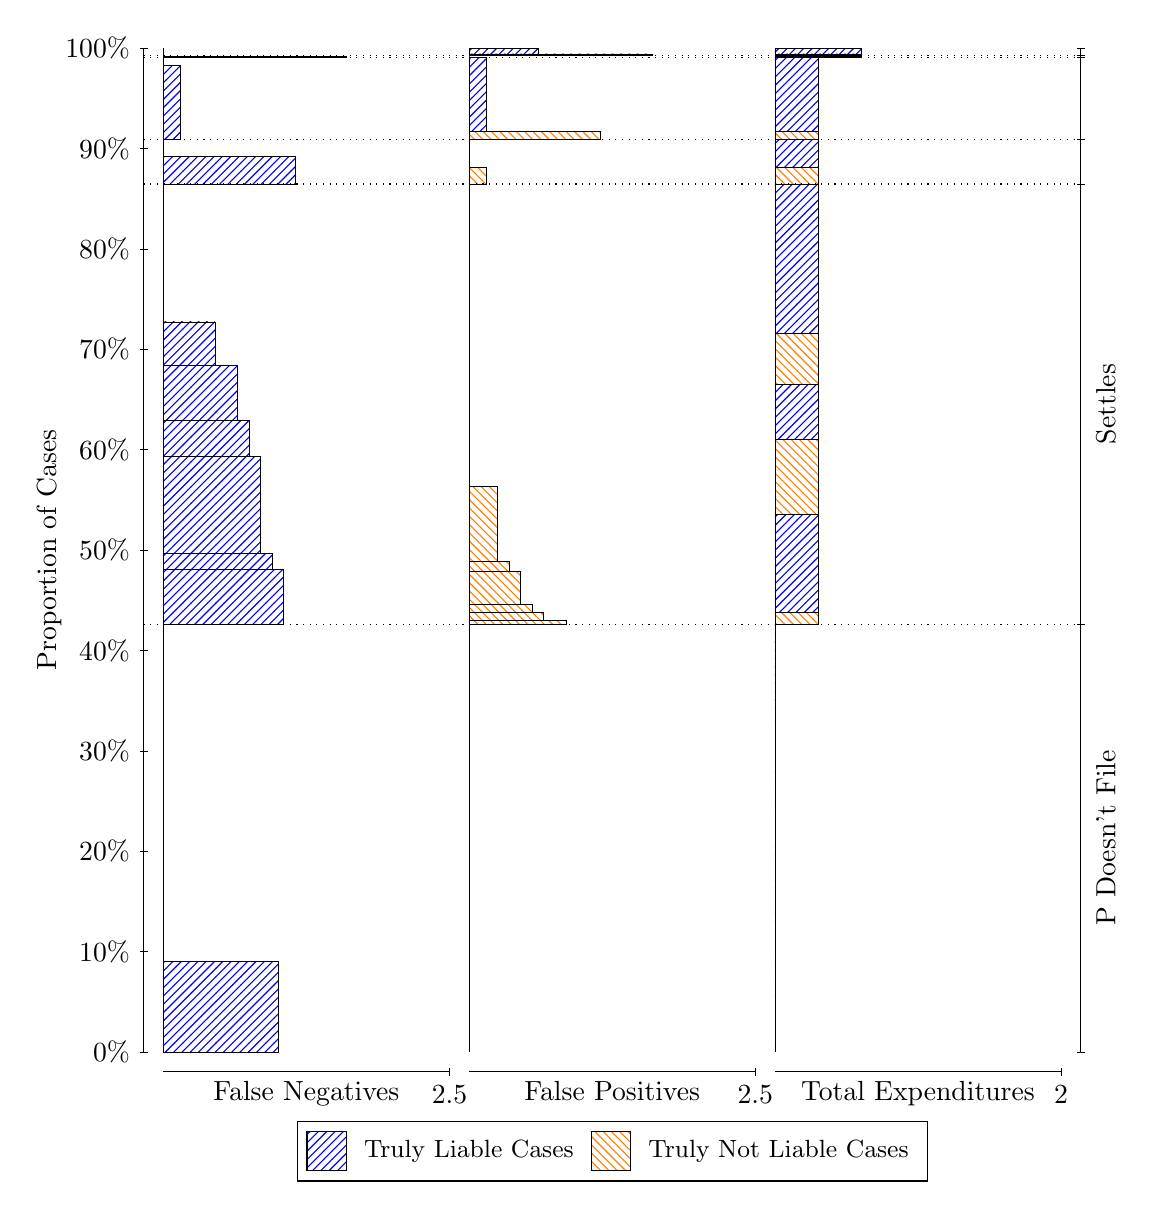
\begin{tikzpicture}
\draw[black, very thin] (1.5,1.75) -- (1.5,14.5);
\node[rotate=90, text=black, anchor=center] at (0.3, 8.125) {Proportion of Cases};
\draw[black, very thin] (1.45,1.75) -- (1.55,1.75);
\node[text=black, anchor=east] at (1.45, 1.75) {0\%};
\draw[black, very thin] (1.45,3.025) -- (1.55,3.025);
\node[text=black, anchor=east] at (1.45, 3.025) {10\%};
\draw[black, very thin] (1.45,4.3) -- (1.55,4.3);
\node[text=black, anchor=east] at (1.45, 4.3) {20\%};
\draw[black, very thin] (1.45,5.575) -- (1.55,5.575);
\node[text=black, anchor=east] at (1.45, 5.575) {30\%};
\draw[black, very thin] (1.45,6.85) -- (1.55,6.85);
\node[text=black, anchor=east] at (1.45, 6.85) {40\%};
\draw[black, very thin] (1.45,8.125) -- (1.55,8.125);
\node[text=black, anchor=east] at (1.45, 8.125) {50\%};
\draw[black, very thin] (1.45,9.4) -- (1.55,9.4);
\node[text=black, anchor=east] at (1.45, 9.4) {60\%};
\draw[black, very thin] (1.45,10.675) -- (1.55,10.675);
\node[text=black, anchor=east] at (1.45, 10.675) {70\%};
\draw[black, very thin] (1.45,11.95) -- (1.55,11.95);
\node[text=black, anchor=east] at (1.45, 11.95) {80\%};
\draw[black, very thin] (1.45,13.225) -- (1.55,13.225);
\node[text=black, anchor=east] at (1.45, 13.225) {90\%};
\draw[black, very thin] (1.45,14.5) -- (1.55,14.5);
\node[text=black, anchor=east] at (1.45, 14.5) {100\%};

\draw[black, very thin] (13.4,1.75) -- (13.4,14.5);
\draw[black, very thin] (13.35,1.75) -- (13.45,1.75);
\node[anchor=west] at (13.35, 1.75) {};
\draw[black, very thin] (13.35,7.1833) -- (13.45,7.1833);
\node[anchor=west] at (13.35, 7.1833) {};
\draw[black, very thin] (13.35,12.773) -- (13.45,12.773);
\node[anchor=west] at (13.35, 12.773) {};
\draw[black, very thin] (13.35,13.339) -- (13.45,13.339);
\node[anchor=west] at (13.35, 13.339) {};
\draw[black, very thin] (13.35,14.38) -- (13.45,14.38);
\node[anchor=west] at (13.35, 14.38) {};
\draw[black, very thin] (13.35,14.41) -- (13.45,14.41);
\node[anchor=west] at (13.35, 14.41) {};
\draw[black, very thin] (13.35,14.5) -- (13.45,14.5);
\node[anchor=west] at (13.35, 14.5) {};

\draw[black, very thin, pattern color=blue, pattern=north east lines] (1.75,1.75) rectangle (3.2033,2.9051);
\draw[black, very thin, pattern color=orange, pattern=north west lines] (1.75,2.9051) rectangle (1.75,7.1833);
\draw[black, very thin, pattern color=blue, pattern=north east lines] (1.75,7.1833) rectangle (3.276,7.8813);
\draw[black, very thin, pattern color=blue, pattern=north east lines] (1.75,7.8813) rectangle (3.1307,8.0834);
\draw[black, very thin, pattern color=blue, pattern=north east lines] (1.75,8.0834) rectangle (2.9853,9.31);
\draw[black, very thin, pattern color=blue, pattern=north east lines] (1.75,9.31) rectangle (2.84,9.7738);
\draw[black, very thin, pattern color=blue, pattern=north east lines] (1.75,9.7738) rectangle (2.6947,10.469);
\draw[black, very thin, pattern color=blue, pattern=north east lines] (1.75,10.469) rectangle (2.404,11.021);
\draw[black, very thin, pattern color=orange, pattern=north west lines] (1.75,11.021) rectangle (1.75,12.773);
\draw[black, very thin, pattern color=blue, pattern=north east lines] (1.75,12.773) rectangle (3.4213,13.126);
\draw[black, very thin, pattern color=orange, pattern=north west lines] (1.75,13.126) rectangle (1.75,13.339);
\draw[black, very thin, pattern color=blue, pattern=north east lines] (1.75,13.339) rectangle (1.968,14.278);
\draw[black, very thin, pattern color=orange, pattern=north west lines] (1.75,14.278) rectangle (1.75,14.38);
\draw[black, very thin, pattern color=blue, pattern=north east lines] (1.75,14.38) rectangle (4.0753,14.396);
\draw[black, very thin, pattern color=orange, pattern=north west lines] (1.75,14.396) rectangle (1.75,14.41);
\draw[black, very thin, pattern color=orange, pattern=north west lines] (1.75,14.41) rectangle (1.75,14.426);
\draw[black, very thin, pattern color=blue, pattern=north east lines] (1.75,14.426) rectangle (1.75,14.5);
\draw[black, very thin, pattern color=orange, pattern=north west lines] (5.6333,1.75) rectangle (5.6333,6.0282);
\draw[black, very thin, pattern color=blue, pattern=north east lines] (5.6333,6.0282) rectangle (5.6333,7.1833);
\draw[black, very thin, pattern color=orange, pattern=north west lines] (5.6333,7.1833) rectangle (6.8687,7.236);
\draw[black, very thin, pattern color=orange, pattern=north west lines] (5.6333,7.236) rectangle (6.578,7.3307);
\draw[black, very thin, pattern color=orange, pattern=north west lines] (5.6333,7.3307) rectangle (6.4327,7.4336);
\draw[black, very thin, pattern color=orange, pattern=north west lines] (5.6333,7.4336) rectangle (6.2873,7.8527);
\draw[black, very thin, pattern color=orange, pattern=north west lines] (5.6333,7.8527) rectangle (6.142,7.9807);
\draw[black, very thin, pattern color=orange, pattern=north west lines] (5.6333,7.9807) rectangle (5.9967,8.9347);
\draw[black, very thin, pattern color=blue, pattern=north east lines] (5.6333,8.9347) rectangle (5.6333,12.773);
\draw[black, very thin, pattern color=orange, pattern=north west lines] (5.6333,12.773) rectangle (5.8513,12.986);
\draw[black, very thin, pattern color=blue, pattern=north east lines] (5.6333,12.986) rectangle (5.6333,13.339);
\draw[black, very thin, pattern color=orange, pattern=north west lines] (5.6333,13.339) rectangle (7.3047,13.441);
\draw[black, very thin, pattern color=blue, pattern=north east lines] (5.6333,13.441) rectangle (5.8513,14.38);
\draw[black, very thin, pattern color=orange, pattern=north west lines] (5.6333,14.38) rectangle (5.6333,14.393);
\draw[black, very thin, pattern color=blue, pattern=north east lines] (5.6333,14.393) rectangle (5.6333,14.41);
\draw[black, very thin, pattern color=orange, pattern=north west lines] (5.6333,14.41) rectangle (7.9587,14.426);
\draw[black, very thin, pattern color=blue, pattern=north east lines] (5.6333,14.426) rectangle (6.5053,14.5);
\draw[black, very thin, pattern color=orange, pattern=north west lines] (9.5167,1.75) rectangle (9.5167,6.0282);
\draw[black, very thin, pattern color=blue, pattern=north east lines] (9.5167,6.0282) rectangle (9.5167,7.1833);
\draw[black, very thin, pattern color=orange, pattern=north west lines] (9.5167,7.1833) rectangle (10.062,7.3307);
\draw[black, very thin, pattern color=blue, pattern=north east lines] (9.5167,7.3307) rectangle (10.062,8.5781);
\draw[black, very thin, pattern color=orange, pattern=north west lines] (9.5167,8.5781) rectangle (10.062,9.5322);
\draw[black, very thin, pattern color=blue, pattern=north east lines] (9.5167,9.5322) rectangle (10.062,10.23);
\draw[black, very thin, pattern color=orange, pattern=north west lines] (9.5167,10.23) rectangle (10.062,10.88);
\draw[black, very thin, pattern color=blue, pattern=north east lines] (9.5167,10.88) rectangle (10.062,12.773);
\draw[black, very thin, pattern color=orange, pattern=north west lines] (9.5167,12.773) rectangle (10.062,12.986);
\draw[black, very thin, pattern color=blue, pattern=north east lines] (9.5167,12.986) rectangle (10.062,13.339);
\draw[black, very thin, pattern color=orange, pattern=north west lines] (9.5167,13.339) rectangle (10.062,13.441);
\draw[black, very thin, pattern color=blue, pattern=north east lines] (9.5167,13.441) rectangle (10.062,14.38);
\draw[black, very thin, pattern color=orange, pattern=north west lines] (9.5167,14.38) rectangle (10.607,14.393);
\draw[black, very thin, pattern color=blue, pattern=north east lines] (9.5167,14.393) rectangle (10.607,14.41);
\draw[black, very thin, pattern color=orange, pattern=north west lines] (9.5167,14.41) rectangle (10.607,14.426);
\draw[black, very thin, pattern color=blue, pattern=north east lines] (9.5167,14.426) rectangle (10.607,14.5);
\draw[black, dotted] (1.5,7.1833) -- (13.4,7.1833);
\draw[black, dotted] (1.5,12.773) -- (13.4,12.773);
\draw[black, dotted] (1.5,13.339) -- (13.4,13.339);
\draw[black, dotted] (1.5,14.38) -- (13.4,14.38);
\draw[black, dotted] (1.5,14.41) -- (13.4,14.41);
\draw[black, very thin] (1.75,1.5) -- (5.3833,1.5);
\node[text=black, anchor=north] at (3.5667, 1.5) {False Negatives};
\draw[black, very thin] (5.3833,1.45) -- (5.3833,1.55);
\node[text=black, anchor=north] at (5.3833, 1.45) {2.5};

\draw[black, very thin] (5.6333,1.5) -- (9.2667,1.5);
\node[text=black, anchor=north] at (7.45, 1.5) {False Positives};
\draw[black, very thin] (9.2667,1.45) -- (9.2667,1.55);
\node[text=black, anchor=north] at (9.2667, 1.45) {2.5};

\draw[black, very thin] (9.5167,1.5) -- (13.15,1.5);
\node[text=black, anchor=north] at (11.333, 1.5) {Total Expenditures};
\draw[black, very thin] (13.15,1.45) -- (13.15,1.55);
\node[text=black, anchor=north] at (13.15, 1.45) {2};

\node[text=black, centered, rotate=90] at (13.72, 4.4667) {P Doesn't File};
\node[text=black, centered, rotate=90] at (13.72, 9.978) {Settles};





\draw (7.449999999999999,1.5) node[draw=none] (baseCoordinate) {};
\begin{scope}[align=center]
        \matrix[scale=0.5, draw=black, below=0.5cm of baseCoordinate, nodes={draw}, column sep=0.1cm]{
            \node[rectangle, draw, minimum width=0.5cm, minimum height=0.5cm, pattern color=blue, pattern=north east lines] {}; &
            \node[draw=none, font=\small, text=black] (B) {Truly Liable Cases}; &
            \node[rectangle, draw, minimum width=0.5cm, minimum height=0.5cm, pattern color=orange, pattern=north west lines] {}; &
            \node[draw=none, font=\small, text=black] (B) {Truly Not Liable Cases}; \\
            };
\end{scope}

\end{tikzpicture}
\end{document}